\section{Results}
\label{sec:results}

\subsection{Genetic Correlation}
\label{sub:psych_genetic_correlation}

Foremost, the genetic correlations betwee impulsive aggression and depressive symptomes is remarkably high ($r_g=0.6741$, $SE=0.0919$, $p=2.2326e-13$).
This high correlation is also reflected in a subjects diagnosed with a major depression ($r_g=0.4134$, $SE=0.1212$, $p=6e-04$).
In contrast, correlations between impulsive aggression and Bipolar disorder did not reached significant levels ($r_g=0.1192$, $SE=0.0949$, $p=0.2091$), and genetic correlations with Schizophrenia, while significant, was not of large effect ($r_g=0.161$, $SE=0.0566$, $p=0.0045$).


In contrast to impulsive aggression, correlations between risk taking and Bipolar ($r_g=0.2561$, $SE=0.0606$, $p=2.4034e-05$), as well as Schizophrenia ($r_g=0.232$, $SE=0.0431$, $p=7.3554e-08$) remain significant after adjusting for multiple testing.
In addition, while genetic correlations were highly significant between aggression and depression, genetic correlations between risk raking, depressive symptomes ($r_g=0.0856$, $SE=0.0687$, $p=0.2129$) as well as MD ($r_g=0.0028$, $SE=0.0853$, $p=0.974$) were small and did not pass the multple testing thershold.


\begin{figure}[htpb]
  \centering
  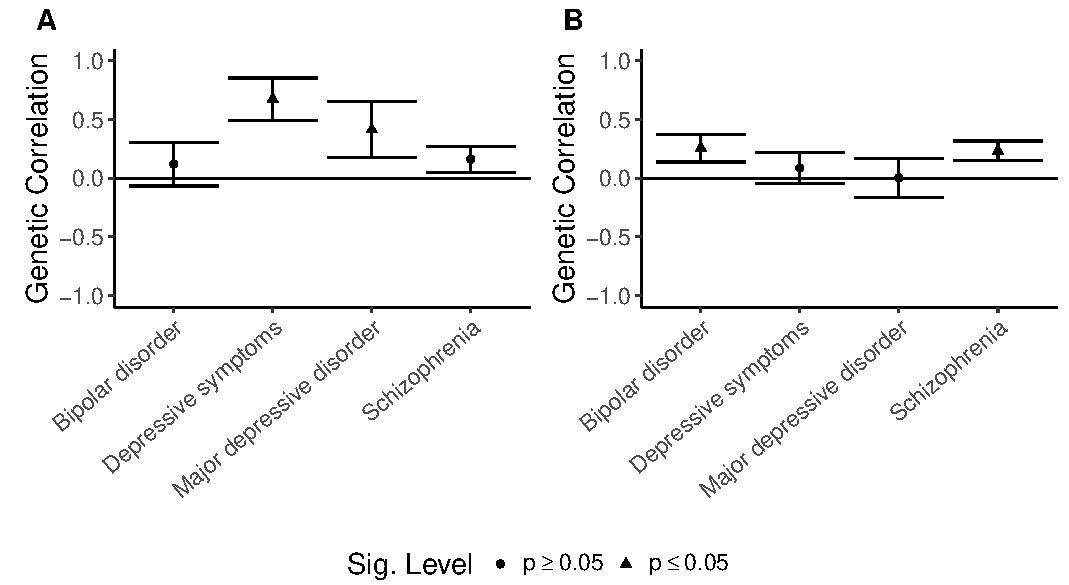
\includegraphics[width=0.8\linewidth]{figures/combined_corr.pdf}
  \caption{Genetic correlations between impulsive aggression and risk taking with selected psychiatric disorders.
    (A) Genetic correlations between impulsive aggrsesion and psychiatric disorders. 
    (B) Genetic correlations between risk taking and psychiatric disorders.
    The error bars display the 95\% confidence intervals for each pairwise genetic correlations.
    Significance levels after multiple testing correction are displayed in form of a dot ($p\ge 0.05$) and triangle ($p\leq0.05$).
  }\label{fig:figures/combined_corr}
\end{figure}

\subsection{Mendelian Randomization}
\label{sub:mendelian_randomization}

Applied MR-method suggest some indication for a causal effect on depressive symptomes as well as MD on impulsive aggression (Figure~\ref{fig:overall_mr_effect}).

\begin{figure}[htpb]
  \centering
  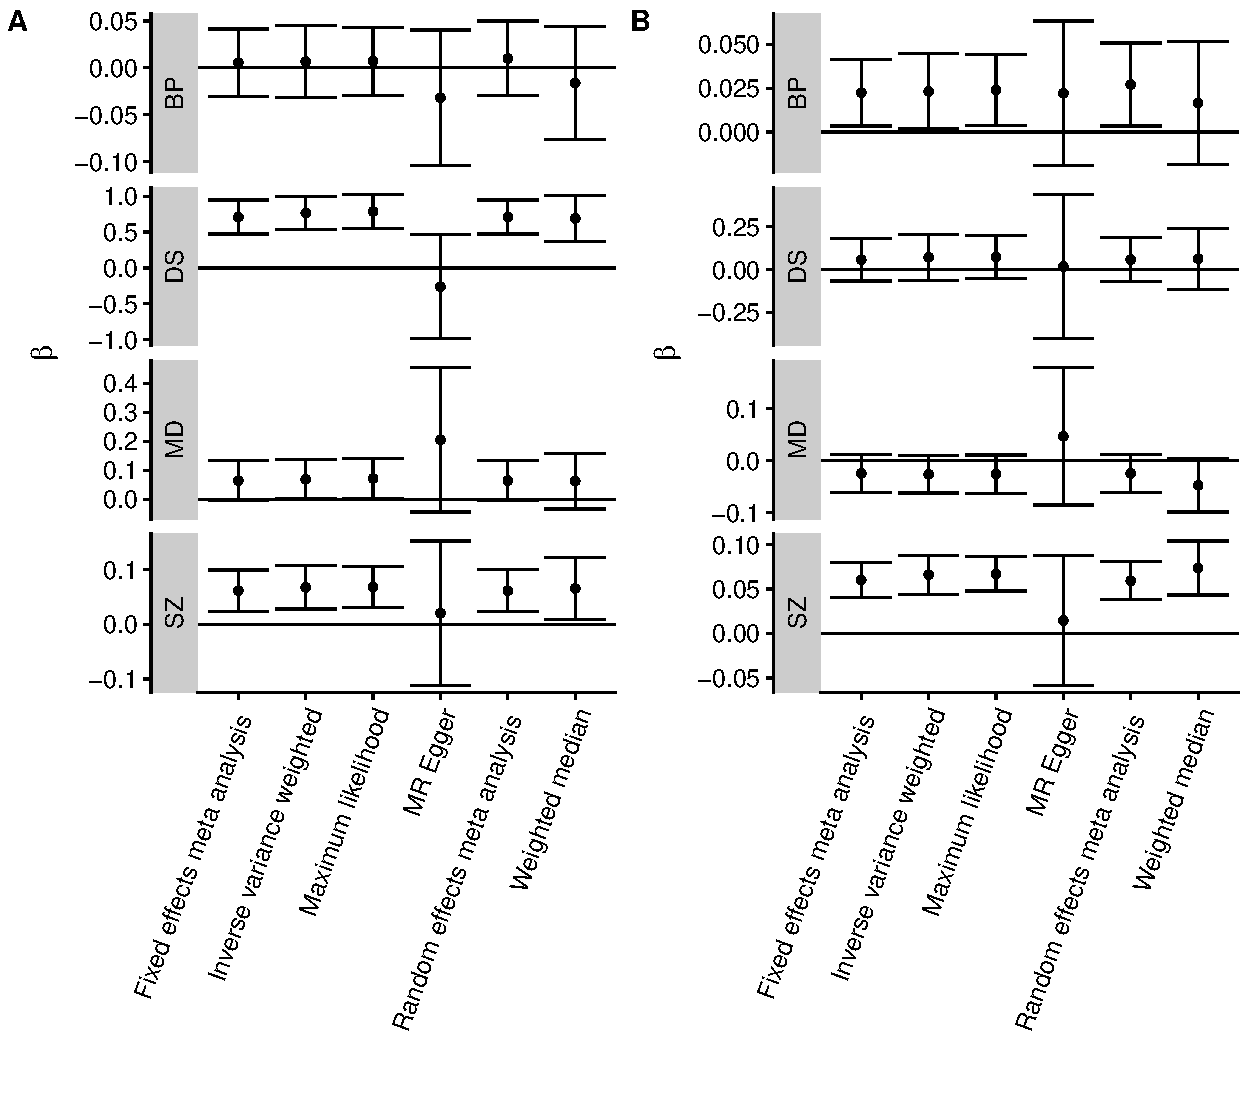
\includegraphics[width=0.9\linewidth]{figures/overall_mr_effect.pdf}
  \caption{Estimated causal effect of psychiatric disorders on impulsive aggression and risk taking.
    The effect size of the causal effect $\beta$ is displayed on the y-axis, while used Mendelian randomization methods are on the x-axis.
    SZ, Schizophrenia; MD, Major Depressive Disorder; DS, Depressive Symptomes; BP, Bipolar Disorder.
    (A) Effect of psychiatric disorders on impulsive aggression.
    (A) Effect of psychiatric disorders on risk taking.
  }\label{fig:overall_mr_effect}
\end{figure}
